\chapter{随机变量的数值特征}
\begin{introduction}[考试重点]
    \item 重期望公式
    \item 重方差公式
    \item 切比雪夫不等式
\end{introduction}

\begin{definition}[期望]
    对于实值随机向量$X :(\Omega,\mathscr{F},\P) \to(\R,\mathscr{B}_{\R})$和(可测)函数$g : \Rn \to \R$,若
    \[ \E[g(X)] = \int_{\R} g(x) \mathrm{d} F_X(x) \]
    存在,则称其为$g(X)$的\textbf{期望}(expectation)。
\end{definition}

\begin{remark}
    当$F_X(x)$在$x_0$初连续可导时,$\mathrm{d} F_X(x_0)=f_X(x_0)\d x$;当$x_0$为其间断点时时,$\d F_X(x_0)=p_X(x_0)\delta(x_0)\d x$。
\end{remark}

%期望算子$\E$是一个线性泛函, 仅适用于\underline{可积}的随机变量.

\begin{theorem}
    对于实值随机向量$X :(\Omega,\mathscr{F},\P) \to(\R,\mathscr{B}_{\R})$和(可测)函数$g : \Rn \to \R$,设 $Y=g(X)$,则有
    \[ \E[g(X)] = \E[Y] \]
\end{theorem}
\begin{proof}
    TODO
\end{proof}

\begin{proposition}[期望的线性性质]
    由积分的线性性质可得:均值为随机变量的线性映射,即
    \[ \E(a+\sum_{i=1}^n b_i g(X_i))=a+\sum_{i=1}^n b_i \E(g(X_i)) \]
\end{proposition}

\begin{proposition}[独立变量的期望]
    若$X,Y$\underline{独立},则
    \begin{gather*}
        \E(XY)=\E(X)\E(Y) \\
        \E(g(X)h(Y))=\E(g(X))\E(h(Y))
    \end{gather*}
\end{proposition}

\begin{remark}
    由于$\E(X/Y)= \E(X)\E(\frac1{Y})$, 而$\E(\frac1{Y}) \neq \frac1{\E(Y)}$, 所以$\E(X/Y)\neq \E(X)/\E(Y)$
\end{remark}

\section{均值与方差}

\begin{definition}
    \begin{enumerate}
        \item 当$g(x)=x$时,$\E[g(x)]=\E[X]$称作$X$的\textbf{均值}(mean),记为$\mu_X$
        \item 当$g(x)=(x-\mu_X)^{2}$时,$\E[g(x)]=\E[(X-\E[X])^{2}]$称作$X$的\textbf{方差}(variance),记为$\sigma^2_X$。其平方根称作$X$的\textbf{标准差}(standard deviation),记为$\sigma_X$
        \item 当$g(x,y)=(x-\mu_X)(y-\mu_Y)$时,$\E[g(X,Y)]=\E[(X-\E[X])(Y-\E[Y])]$称作$X$与$Y$的\textbf{协方差}(covariance),记为$\Cov(X,Y)$或$\sigma_{XY}$
    \end{enumerate}
\end{definition}

\subsection{均值}

随机变量的均值可看作其加权平均,权重为其pdf或pmf,结果为其函数图像上的形心。从大数定律(第\ref{sec:large_number}节)的角度看,也可解释为其长期均值。

\begin{example}
    在一个人数为$N$的人群中普查某种疾病,为此要抽验$N$个人的血。如果将每个人的血分别检验,则共需检验$N$次。为了能减少工作量,一位统计学家提出一种方法:按$k$个人一组进行分组,把同组$k$个人的血样混合后检验,如果这混合血样呈阴性反应,就说明此$k$个人的血都呈阴性反应,此$k$个人都无此疾病,因而这$k$个人只要检验1次就够了,相当于每个人检验$1/k$次,检验的工作量明显减少了。如果这混合血样呈阳性反应,就说明此$k$个人中至少有一人的血呈阳性反应,则再对此$k$个人的血样分别进行检验,因而这$k$个人的血要检验$1+k$次,相当于每个人检验$1+1/k$次,这时增加了检验次数。假设该疾病的发病率为$p$,且得此疾病相互独立。试问此种方法能否减少平均检验次数?
\end{example}
\begin{solution}
    令$X$为该人群中每个人需要的验血次数,则$X$的分布列为
    \begin{table}[htbp]
        \centering
        \begin{tabular}{c|cc}
            $x$ & $1 / k$   & $1+1 / k$   \\\midrule
            $P$ & $(1-p)^k$ & $1-(1-p)^k$ \\
        \end{tabular}
    \end{table}
    所以每人平均验血次数为
    \[ E(X)=\frac1{k}(1-p)^k+(1+\frac1{k})[1-(1-p)^k]=1-(1-p)^k+\frac1{k} \]
    由此可知,只要选择$k$使
    \[ 1-(1-p)^k+\frac1{k}<1,\ \text{即},\ (1-p)^k>\frac1{k} \]
    就可减少验血次数,而且还可适当选择$k$使其达到最小。
\end{solution}

\begin{example}[凑一法求解二项分布的均值]\label{ex:binom_dist_mean}
    求解二项分布(定义\ref{def:binom_dist})的均值时,可通过将其凑成概率质量函数之和(为1)的形式,称此为\textbf{凑一法}(sum to one, STO):
    \begin{align*}
        E(X) & =\sum_{i=1}^n x \binom{n}{x} p^x(1-p)^{n-x}                 \\
             & = np \sum_{i=1}^n \binom{n-1}{x-1} p^{x-1}(1-p)^{n-1-(x-1)} \\
             & =np
    \end{align*}
\end{example}

\begin{example}[微分法求解几何分布均值]\label{ex:geometric_dist_mean}
    \begin{align*}
        E(X) & =p\sum_{k=1}^{\infty}k q^{k-1}=p\frac{d}{d q}\sum_{k=1}^{\infty} q^{k} \\
             & =p\frac{d}{d q} \frac{q}{1-q} =\frac{p}{(1-p)^{2}}                     \\
             & =\frac{1}{p}                                                           \\
    \end{align*}
\end{example}

\begin{proposition}\label{prop:mean_of_non-negative_discrete_varible}
    设$X$为仅取非负整数的离散随机变量,若其数学期望存在,则
    \[ E(X) = \sum_{k=1}^{+\infty}P(X \ge k) \]
\end{proposition}

\subsection{方差}

方差为随机变量距其均值的均方偏差,刻画了$X$的变动程度。随机变量的均值与标准差的单位和其本身的相同,方差的为其平方。如果随机变量$X$的数学期望存在, 其方差不一定存在;而当$X$的方差存在时,则$E(X)$必定存在,其原因在于$|x| \le x^2+1$($0 \le x^2-2|x|+1$)总是成立的(若$E(X^2)$收敛,则$E(|X|)$收敛)。

\begin{proposition}
    \[ \operatorname{Var}(X)=\E[(X-\mu_X)^2]=E(X^2)-\mu_X \]
\end{proposition}

\begin{example}[凑一法求解二项分布的方差]\label{ex:binom_dist_var}
    \begin{align*}
        E(X(X-1))             & =\sum_{i=1}^n x(x-1) \binom{n}{x} p^x(1-p)^{n-x}                   \\
                              & = n(n-1)p^2 \sum_{i=1}^n \binom{n-2}{x-2} p^{x-2}(1-p)^{n-1-(x-1)} \\
                              & =n(n-1)p^2                                                         \\
        \operatorname{Var}(X) & =  E(X(X-1)) + E(X) -(E(X))^2                                      \\
                              & = n(n-1)p^2 + np -n^2 p^2                                          \\
                              & =np(1-p)
    \end{align*}
\end{example}

\begin{example}[微分法求解几何分布方差]\label{ex:geometric_dist_var}
    \begin{align*}
        E(X(X-1))             & =p\sum_{k=1}^{\infty}k(k-1) q^{k-1}=p\frac{d}{d q}\sum_{k=1}^{\infty} q^{k} \\
                              & =p\frac{d^2}{d q^2} \frac{q}{1-q} =\frac{2p}{(1-q)^{3}}                     \\
                              & =\frac{2}{p^2}                                                              \\
        \operatorname{Var}(X) & =  E(X(X-1)) + E(X) -(E(X))^2                                               \\
                              & = \frac{2}{p^2} + \frac{1}{p} -\frac{1}{p^2} p^2                            \\
                              & = \frac{1-p}{p^2}
    \end{align*}
\end{example}

\begin{proposition}
    \[ \operatorname{Var}(a+bX)=b^2\operatorname{Var}(X) \]
\end{proposition}

\begin{proposition}
    \[ \operatorname{Var}(a+\sum_{i=1}^n b_i X_i)=\mathbf{b}^{\mathrm{T}} \Sigma \mathbf{b}\]
    其中$\Sigma$为协方差矩阵,$\Sigma_{i,j}=\operatorname{Cov}(X_i,X_j)$
\end{proposition}
\begin{proof}
    由方差的定义知
    \begin{align*}
        \Var(X \pm Y) & =E\{(X \pm Y)-E(X \pm Y)\}^2                      \\
                      & =E\{(X-E(X)) \pm(Y-E(Y))\}^2                      \\
                      & =E\{(X-E(X))^2+(Y-E(Y))^2 \pm 2(X-E(X))(Y-E(Y))\} \\
                      & =\Var(X)+\Var(Y) \pm 2 \Cov(X, Y)
    \end{align*}
\end{proof}

\begin{corollary}
    若$X_1,\cdots ,X_n$相互不相关,则:
    \[ \operatorname{Var}(\sum_{i=1}^n X_i)=\sum_{i=1}^n\operatorname{Var}(X_i) \]
\end{corollary}

\begin{theorem}[Chebyshev不等式]
    设随机变量$X$的均值与方差分别为:$\mu, \sigma^2$, 则:
    \[ \P(\left| X-\mu \right| >t)\le \frac{\sigma^{2}}{t^{2}} \]
\end{theorem}

\begin{proof}
    设$F(x)$为$X$的分布函数, 令$R=\left\{ x:|x-\mu|>t \right\}$
    \begin{align*}
        \P(|x-\mu|>t) & = \int_R 1 \cdot  \d F(x) \le \int_R \frac{(x-\mu)^2}{t^{2}}\d F(x)                   \\
                      & \le \int_{-\infty}^{\infty}\frac{(x-\mu)^2}{t^{2}}\d F(x)  = \frac{\sigma^{2}}{t^{2}}
    \end{align*}
    再由协方差的运算性质(命题\ref{prop:cov_property}),通过数学归纳法可推出泛化的结果。
\end{proof}

\begin{remark}
    若令$t=k\sigma$, 则$\P(| X-\mu | >k\sigma)\le \frac1{k^{2}}$, 即标准差可代表随机变量偏离均值的概率单位距离.
\end{remark}

\begin{corollary}\label{cor:var_almost_equal}
    \[ \operatorname{Var}(X)=0 \Leftrightarrow P(X=\mu)=1 \]
\end{corollary}

预处理随机变量有两个常用变换:
\begin{itemize}
    \item \textbf{中心化}(centralization)$X \mapsto X-\E{X}$;
    \item \textbf{标准化}(standardization)$X \mapsto \dfrac{X-\E{X}}{\sqrt{\Var(X)}}$.
\end{itemize}

\section{协方差与相关系数}

\subsection{协方差}

协方差代表了$X$与$Y$之间的联合变化倾向,或者说他们间的相关程度,但其间\underline{未必有}因果关系。
\begin{itemize}
    \item 若$\operatorname{Cov}(X,Y) >0$,则称两变量\textbf{正相关};
    \item 若$\operatorname{Cov}(X,Y) < 0$,则称两者\textbf{负相关};
    \item 若$\operatorname{Cov}(X,Y) = 0$,则称两者\textbf{不相关}。
\end{itemize}

\begin{remark}
    不相关是指$X$与$Y$之间没有线性关系,但$X$与$Y$之间可能有其他的函数关系,譬如平方关系、对数关系等。
\end{remark}

\begin{proposition}
    \[ \operatorname{Cov}(X,Y)=\E[(X-\mu_X)(Y-\mu_Y)]=\E(XY)-\mu_Y \mu_Y \]
\end{proposition}

\begin{proposition}
    独立是不相关的\textbf{充分条件},但不是必要条件。
\end{proposition}
\begin{example}\label{exam:3.4.6}
    设随机变量$X \sim N(0,\sigma^2)$,令$Y=X^2$,则$X$与$Y$不独立。此时$X$与$Y$的协方差为
    \[ \Cov(X, Y)=\Cov(X, X^2)=E(X\cdot X^2)-E(X)E(X^2) \]
    由于正态分布$N(0,\sigma^2)$的奇数阶原点矩均为零,即$E(X)=E(X^3)=0$,故上式也等于零。
\end{example}

“独立”必导致“不相关”;而“不相关”不一定导致“独立”。因为独立性是用分布定义的,而不相关只是用矩定义的。

\begin{proposition}
    若 $X, Y$皆为二值随机变量,则不相关性与独立性等价。
\end{proposition}
\begin{proof}
    设
\end{proof}

\begin{proposition}\label{prop:cov_property}
    协方差的运算性质:
    \begin{itemize}
        \item 协方差$\Cov(X,Y)$的计算与$X,Y$的次序无关
              \[ \Cov(X,Y)=\Cov(Y,X) \]
        \item 任意随机变量$X$与常数$a$的协方差为零
              \[ \Cov(X,a)=0 \]
        \item 对任意常数$a,b$,有
              \[ \Cov(a X, b Y)=a b \Cov(X, Y) \]
        \item 设$X,Y,Z$是任意三个随机变量, 则
              \[ \Cov(X+Y, Z)=\Cov(X, Z)+\Cov(Y, Z) \]
    \end{itemize}
\end{proposition}

\begin{corollary}
    线性变换后的协方差:
    \begin{gather*}
        \operatorname{Cov}(a+ b X,c +d Y)  = b d \Cov(X,Y)\\
        \operatorname{Cov}(a+\sum_{i=1}^n b_i X_i,c+\sum_{j=1}^m d_j Y_j) = \sum_{i=1}^n\sum_{j=1}^m b_i d_j \operatorname{Cov}(X_i,Y_i) = \mathbf{b}^{\mathrm{T}}\Sigma \mathbf{d}
    \end{gather*}
\end{corollary}

\begin{definition}[协方差矩阵]
    对于$n$维随机向量$\mathbf{X}=(X_1,X_2,\ldots,X_n)'$,将
    \begin{align*}
         & E[(\mathbf{X}-E(\mathbf{X}))(\mathbf{X}-E(\mathbf{X}))' ] \\
         & =\begin{pmatrix}
                \Var(X_1)     & \Cov(X_1,X_2) & \cdots & \Cov(X_1,X_n) \\
                \Cov(X_2,X_1) & \Var(X_2)     & \cdots & \Cov(X_2,X_n) \\
                \vdots        & \vdots        &        & \vdots        \\
                \Cov(X_n,X_1) & \Cov(X_n,X_2) & \cdots & \Var(X_n)
            \end{pmatrix}
    \end{align*}
    称为该随机向量的\textbf{方差—协方差阵},简称\textbf{协方差阵},记为$\Sigma=\Cov(\mathbf{X})$。
\end{definition}

\begin{theorem}
    $n$维随机向量的协方差阵$\Cov(\mathbf{X})=(\Cov(X_i,X_j))_{n\times n}$是一个对称的非负定矩阵。
\end{theorem}
\begin{proof}
    因为$\Cov(X_i,X_j)=\Cov(X_j,X_i)$,所以对称性是显然的。下证非负定性。因为对任意$n$维实向量$\mathbf{c}=(c_1,\cdots ,c_n)'$,有
    \begin{align*}
        \mathbf{c}'\Cov(\mathbf{X})\mathbf{c} & = \sum_{i=1}^n\sum_{j=1}^n c_i c_j \Cov(X_i,X_j)                                                                           \\
                                              & = \sum_{i=1}^n\sum_{j=1}^n E\{ [c_i(X_i-E(X_i))] [c_j(X_j-E(X_j))] \}                                                      \\
                                              & = E\left\{\sum_{i=1}^n \sum_{j=1}^n [c_i\left(X_i-E\left(X_i\right)\right)][c_j\left(X_j-E\left(X_j\right)\right)]\right\} \\
                                              & = E\left\{\left[\sum_{i=1}^n c_i(X_i-E(X_i))\right]\left[\sum_{j=1}^n  c_j(X_j-E(X_j))\right]\right\}                      \\
                                              & = E\left[\sum_{i=1}^n  c_i(X_i-E(X_i))\right]^2 \ge 0
    \end{align*}
    所以矩阵$\Cov(\mathbf{X})$是非负定的。
\end{proof}

\subsection{相关系数}

\begin{definition}
    设$(X,Y)$是一个二维随机变量, 且$\Var(X)>0,\Var(Y)>0$。则称
    \[ \Corr(X,Y)=\frac{\sigma_{XY}}{\sigma_X\sigma_Y} \]
    为$X$与$Y$的(线性)\textbf{相关系数}(correlation coefficient),可简记为$\rho_{XY}$。
\end{definition}


相关系数是相应标准化变量的协方差。若记$X$与$Y$的数学期望分别为$\mu_X,\mu_Y$,其标准化变量为:
\[ X^*=\frac{X-\mu_X}{\sigma_X},\quad Y^*=\frac{Y-\mu_Y}{\sigma_Y} \]
则有
\[ \Cov(X^*, Y^*)=\Cov\left(\frac{X-\mu_X}{\sigma_X}, \frac{Y-\mu_Y}{\sigma_Y}\right)=\frac{\Cov(X, Y)}{\sigma_X\sigma_Y}=\Corr(X, Y) \]

\begin{proposition}
    平移与缩放随机变量都不影响其相关系数的绝对值,但其是否变号取决于缩放系数的正负,即:
    \[ \operatorname{Corr}(a+ b X,c +d Y)  = \operatorname{Corr}(X,Y) \operatorname{sign}(b d) \]
\end{proposition}

\begin{example}\label{exam:3.4.9}
    二维正态分布$N(\mu_{1}, \mu_{2}, \sigma_{1}^{2}, \sigma_{2}^{2}, \rho)$的相关系数是$\rho$。
\end{example}
\begin{solution}
    由上述可知,平移与缩放变量不影响两者间相关系数,故不妨将变量标准化:
    \[ X^*=\frac{X-\mu_X}{\sigma_X},\quad Y^*=\frac{Y-\mu_Y}{\sigma_Y} \]
    则其密度函数变为:
    \[ f_{X^*,Y^*}(x,y) = \sigma_X \sigma_Y f_{X,Y}(\sigma_X x+\mu_X,\sigma_Y y+\mu_Y) = \frac{1}{2 \pi \sqrt{1-\rho^2}} \exp \left(- \frac{x^2 - 2 \rho x y +y^2}{2(1-\rho^2)} \right)\]
    \[ E(X^* Y^*) = \frac{1}{2 \pi \sqrt{1-\rho^2}} \int_{-\infty}^{+\infty}\int_{-\infty}^{+\infty}x y \exp \left(- \frac{x^2 - 2 \rho x y +y^2}{2(1-\rho^2)} \right) \d x \d y\]
    做变换:
    \[ \begin{cases}
            u = \frac{x- \rho y}{\sqrt{1-\rho^2}} \\
            v = y
        \end{cases} \implies \begin{cases}
            x = \sqrt{1-\rho^2}u + \rho v \\
            y =  v
        \end{cases} \implies \dd x\dd y= \sqrt{1-\rho^2}\dd u\dd v \]
    由此得
    \[ \Cov(X,Y)=\frac{1}{2\pi}\int_{-\infty}^{+\infty}\int_{-\infty}^{+\infty}(uv\sqrt{1-\rho^2}+\rho v^2)\exp\left\{ -\frac{u^2+v^2}{2} \right\}\dd u\dd v \]
    上式右端积分可以分为两个积分, 其中
    \begin{align*}
         & \int_{-\infty}^{+\infty}\int_{-\infty}^{+\infty} uv\exp\left(-\frac{u^2+v^2}{2} \right)\dd u\dd v=0,     \\
         & \int_{-\infty}^{+\infty}\int_{-\infty}^{+\infty} v^2\exp\left(-\frac{u^2+v^2}{2} \right)\dd u\dd v=2\pi.
    \end{align*}
    从而
    \begin{align*}
        \Cov(X^*,Y^*) & =E(X^* Y^*)=\frac{1}{2\pi}\cdot \rho\cdot 2\pi=\rho \\
        \Corr(X,Y)    & =\Corr(X^*,Y^*)=\frac{\Cov(X,Y)}{1 \cdot 1}=\rho
    \end{align*}
\end{solution}

\begin{lemma}[施瓦茨不等式]
    对任意二维随机变量$(X,Y)$, 若$X$与$Y$的方差都存在, 且记$\sigma_{X}^2=\Var(X),\sigma_{Y}^2=\Var(Y)$, 则有
    \[ [\Cov(X,Y)]^2\leq \sigma_{X}^2\sigma_{Y}^2 \]
\end{lemma}
\begin{proof}
    不妨设$\sigma_{X}^2>0$, 因为当$\sigma_{X}^2=0$时, 则$X$几乎处处为常数, 因而其与$Y$的协方差亦为零, 从而上式两端皆为零, 结论成立. 在$\sigma_{X}^2>0$成立下, 考虑$t$的如下二次函数:
    \[ g(t)=E[t(X-E(X))+(Y-E(Y))]^2=t^2 \sigma_{X}^2+2t\cdot \Cov(X,Y)+\sigma_{Y}^2 \]
    由于上述的二次三项式非负, 平方项系数$\sigma_{X}^2$为正, 所以其判别式小于或等于零, 即
    \[ [2\Cov(X,Y)]^2-4\sigma_{X}^2\sigma_{Y}^2\leq0 \]
    移项后即得施瓦茨不等式.
\end{proof}

\begin{proposition}
    $-1 \le \rho_{XY} \le 1$。取等号的充要条件是$X$与$Y$间几乎处处有线性关系,即存在$a(\ne0)$与$b$,使得:
    \[ P(Y=aX+b)=1 \]
    上式换成$X=cY+d$也一样
\end{proposition}
\begin{proof}
    \textbf{充分性}:若$Y=aX+b$,则有
    \[ \Var(Y)=a^2\Var(X),\Cov(X,Y)=a\Cov(X,X)=a\Var(X) \]
    代入相关系数的定义中得
    \[ \Corr(X,Y)=\frac{\Cov(X,Y)}{\sigma_{X}\sigma_{Y}}=\frac{a\Var(X)}{|a|\Var(X)}=\begin{cases}
            1,  & a>0; \\
            -1, & a<0.
        \end{cases} \]
    \textbf{必要性}:因为
    \[ \Var\left(\frac{X}{\sigma_{X}}\pm\frac{Y}{\sigma_{Y}} \right)=2[1\pm\Corr(X,Y)] \]
    所以当$\Corr(X,Y)=1$时,有
    \[ \Var\left(\frac{X}{\sigma_{X}}-\frac{Y}{\sigma_{Y}} \right)=0 \]
    由此得(推论\ref{cor:var_almost_equal})
    \begin{align*}
         & P\left(\frac{X}{\sigma_{X}}-\frac{Y}{\sigma_{Y}}=c \right)=1  \\
         & P\left(Y=\frac{\sigma_{Y}}{\sigma_{X}}X-c\sigma_{Y} \right)=1
    \end{align*}
    即当$\Corr(X,Y)=1$时,$Y$与$X$几乎处处线性正相关.

    当$\Corr(X,Y)=-1$时, 由同理得
    \[ P\left(Y=-\frac{\sigma_{Y}}{\sigma_{X}}X+c\sigma_{Y} \right)=1 \]
    即当$\Corr(X,Y)=-1$时,$Y$与$X$几乎处处线性负相关.
\end{proof}

\section{不等式}

\subsection{Chebyshev-Markov型不等式}

\begin{theorem}[Markov不等式]\label{thm:Markov_inequality}
    设$g(x)$为随机变量$X$取值的集合上的非负不减函数,且$E(g(X))$存在,则
    \[ P(X>\e) \leq \frac{E(g(X))}{g(\e)} ,\quad \forall \e > 0\]
\end{theorem}
\begin{proof}
    \begin{align*}
        P(X>\e) & =\int_{\e}^{+\infty} \d F(x) \leq \int_{\e}^{+\infty}\frac{g(X)}{g(\e)}\d F(x) \\
                & \leq \int_{-\infty}^{+\infty}\frac{g(X)}{g(\e)}\d F(x) = \frac{E(g(X))}{g(\e)}
    \end{align*}
\end{proof}

\begin{corollary}
    若$g(X) \ge 0$,则
    \[ \E[g(X)] = 0 \Leftrightarrow  \P\{g(X)=0\} = 1 \Leftrightarrow g(X) \overset{\as}{=} 0 \]
\end{corollary}

\begin{proposition}[Chebyshev不等式]
    \[ P\{ \left\vert X-E(X) \right\vert \ge x \} \le \frac{\operatorname{Var}(X)}{x^2}\]
\end{proposition}
\begin{proof}
    令Markov不等式(定理\ref{thm:Markov_inequality})中的$g(x)=x^2$则可得:
    \[ P\{ \left\vert X-E(X) \right\vert \ge x \} = P\{ [X-E(X)]^2 \ge x^2 \} \le \frac{E[X-E(X)]^2}{x^2}=\frac{\operatorname{Var}(X)}{x^2} \]
\end{proof}

\begin{proposition}[Markov不等式]
    \[ P\{ \left\vert X \right\vert \ge x \} \le \frac{E(|X|^r)}{x^r} ,\quad \forall r>0,x>0\]
\end{proposition}
\begin{proof}
    令Markov不等式(定理\ref{thm:Markov_inequality})中的$g(x)=x^r$则可得:
    \[ P\{ \left\vert X \right\vert \ge x \} = P\{ |X|^r \ge x^r \} \le \frac{E(|X|^r)}{x^r} \]
\end{proof}

\begin{proposition}[Chebyshev不等式的推广]\label{prop:Chebyshev_inequality_extend}
    \[ P\{ X-E(X) \ge x \} \le \frac{\sigma^2+a^2}{(x+a)^2} ,\quad \forall x,a\]
\end{proposition}
\begin{proof}
    令Markov不等式(定理\ref{thm:Markov_inequality})中的$g(x)=x$则可得:
    \begin{align*}
        P\{ X-E(X) \ge x \} & =P\{ X-E(X)+a \ge x+a \}                                         \\
                            & \le  P\{ [X-E(X)+a]^2 \ge (x+a)^2 \}                             \\
                            & \le \frac{E[X-E(X)+a]^2}{(x+a)^2} = \frac{\sigma^2+a^2}{(x+a)^2}
    \end{align*}
\end{proof}

\begin{example}[单边Chebyshev不等式]
    设随机变量X的均值为$\mu$,方差为$\sigma^2$,则对于任意$x>0$有:
    \[ P\{ X-\mu\ge x \}\le \frac{\sigma^2}{x^2+\sigma^2} \]
\end{example}
\begin{solution}
    令Chebyshev不等式的推广形式(命题\ref{prop:Chebyshev_inequality_extend})中的$a=\frac{\sigma^2}{x}$,则
    \[ \frac{\sigma^2+a^2}{(x+a)^2}=\frac{\sigma^2+\frac{\sigma^4}{x^2}}{x^2+2\sigma^2+\frac{\sigma^4}{x^2}}=\frac{\sigma^2}{x^2+\sigma^2} \]
\end{solution}

\begin{proposition}[Chebyshev不等式的离散情形]
    设离散随机变量$X$的取值范围为正自然数,且$P\{ X-k \}$非增,则
    \[ P\{ X=k \} < \frac{2}{k^2}E(X) \]
\end{proposition}
\begin{proof}
    \begin{align*}
        E(X) & =\sum_{i=1}^{\infty}i P\{ X=i \} \ge \sum_{i=1}^{k}i P\{ X=i \}                      \\
             & \ge \sum_{i=1}^{k}i P\{ X=k \} = P\{ X=k \} \frac{k(k+1)}{2} \\
             & \ge \frac{k^2}{2}P\{ X=k \}
    \end{align*}
\end{proof}

\subsection{Cauchy-Schwarz不等式}

\begin{proposition}[Cauchy-Schwarz不等式]
    \[ E(|XY|) \le [E(X^2)]^{\frac{1}{2}} [E(Y^2)]^{\frac{1}{2}} \]
\end{proposition}
\begin{proof}
    令$g(t)=E[|X|+t|Y|]^2$,易知其恒大于$0$。又
    \[ g(t)=E[X^2]+2tE(|XY|)+ t^2E[Y^2] \]
    则其判别式
    \[ \Delta = 4E^2(|XY|)-4[E(X^2)] [E(Y^2)] \le 0 \]
\end{proof}

\begin{proposition}[Holder不等式]
    若$p,q$满足$p,q>1,\ \frac{1}{p}+\frac{1}{q}=1 $,则
    \[ E(|XY|) \le [E(X^p)]^{\frac{1}{p}} [E(Y^q)]^{\frac{1}{q}} \]
\end{proposition}

\subsection{Jensen不等式}

\begin{theorem}[Jensen不等式]
    若$g:R \to R$为\underline{下凸(convex)函数},则$g[\E(X)] \le \E[g(X)]$;若$g$为\underline{上凸(concave)函数},则$\E[g(X)] \le g[\E(X)]$。
\end{theorem}
\begin{proof}
    若$g$为下凸函数,则
    \[ g(x)\ge g(x_0)+g'(x-x_0) \]
    令$x_0=E(X)$,得
    \[ g(x)\ge g(E(X))+g'(x-E(X)) \]
    再对两边取期望,得
    \[ E(g(X))\ge g(E(X))+E[g'(X-E(X))]=g(E(X)) \]
\end{proof}

\begin{figure}[h]
    \centering
    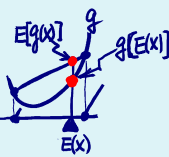
\includegraphics{image/trans_mean.png}
    \caption{设随机变量$X$遵循两点分布,取值为$\{ a,b \}$,此为其变换后各值}
\end{figure}

\begin{lemma}
    \[ (E|X|^r)^{\frac{1}{r}} \le (E|X|^s)^{\frac{1}{s}} ,\quad \forall 0<r \le s \]
\end{lemma}
\begin{proof}
    令$g(x)=x^{\frac{s}{r}}$且$Y=|X|^r$得
    \[ E^{\frac{s}{r}}(Y) \le E(Y^{\frac{s}{r}}) \]
    即
    \[ E^{\frac{s}{r}}(|X|^r) \le E(|X|^s) \]
\end{proof}

\subsection{最小一乘法}

\begin{proposition}
    设随机变量$X$的\underline{均值}为$\mu$,则对任意常数$c$,有
    \[ E(X-\mu)^2 \le E(X-c)^2 \]
\end{proposition}
\begin{proof}
    将$E(X-c)^2=E(X-\mu+\mu-c)^2$展开即可
\end{proof}

\begin{proposition}
    设随机变量$X$的\textbf{中位数}为$m$,则对任意常数$c$,有
    \[ E|X-m| \le E|X-c| \]
\end{proposition}
\begin{proof}
    设 $g(m)=E\abs{X-m}$,则
    \begin{align*}
        E\abs{X-m} &= \int^m_{-\infty}(m-x)\d F(x) + \int_m^{\infty}(x-m)\d F(x) \\
        &= (m-x)F(x)|^m_{-\infty} + \int^m_{-\infty} F(x) \d x + \int_m^{\infty}x\d F(x) - m(1-F(x)) \\
        g'(m) &= F(m) - mF'(m) -1 +F(m)+mF'(m) \\
        &=2F(m)-1
    \end{align*}
    所以,当 $m=F^{-1}(\frac{1}{2})$时,$g(m)$最小,即$m$是$X$的中位数。
\end{proof}

\begin{proposition}
    若$x_1,\cdots ,x_n $是总体$X$的一组样本,其中$x_{med}$为样本中位数,$\overline{x}$是样本均值。则对任意常数$c$有:
    \begin{itemize}
        \item $\sum_{i=1}^n(x_i-\overline{x})^2 \le \sum_{i=1}^n(x_i-c)^2$
        \item $\sum_{i=1}^n|x_i-x_{med}| \le \sum_{i=1}^n|x_i-c|$
    \end{itemize}
\end{proposition}

\section{条件期望}

\begin{definition}
    若$h(Y)$在给定$X=x$下的条件分布(定义\ref{def:cond_dist})的数学期望存在,则定义其为\textbf{条件期望}如下:
    \[ E(h(Y)|X=x) =\begin{cases}
            \sum_y h(y) p_{Y|X}(y|x),                      & \text{离散情况} \\
            \int_{-\infty}^{+\infty} h(y) f_{Y|X}(y|x) d y & \text{连续情况}
        \end{cases}\]
\end{definition}
\begin{remark}
    条件期望$\E_{Y|X}(Y|x)$是关于给定变量$x$的函数,不随对应变量$Y$本身变动,但其单位与对应变量$Y$相同,可看作一条在$(X,Y)$平面的曲线。
\end{remark}

\begin{proposition}
    若随机变量$X,Y$独立,则:
    \[ \E_{Y|x}(Y|x)=\E_Y(Y) \]
\end{proposition}
\begin{proof}
    由定理\ref{thm:indep_cmf}可知,若随机变量$X,Y$独立,则
    \begin{align*}
        p_{Y|X}(y|x) & =p_Y(y) \\
        f_{Y|X}(y|x) & =f_Y(y)
    \end{align*}
    所以$\E_{Y|x}(Y|x)=\E_Y(Y)$
\end{proof}
由直观感受亦可知:若$X,Y$独立,则$X$不通过任何与$Y$相关的信息,其条件期望亦当与原期望相同。

若令$g(x)=\E(h(Y)|X=x)$,则$g(X)$是随机变量$X$的变换,也是随机变量,记为$\E(h(Y)|X)$。

\begin{theorem}[重期望公式]
    \[ \E_Y[h(Y)] = \E_X[\E_{Y|X}(h(Y)|X)] \]
\end{theorem}
\begin{proof}
    设二维连续随机变量$(X,Y)$的联合密度函数为$f(x,y)$。利用$f(x,y)=f_{y|x}(y|x)f_X(x)$,可得:
    \begin{align*}
        \E_Y[h(Y)] & = \int_{-\infty}^{+\infty} \int_{-\infty}^{+\infty} h(y) f(x, y) \dd x \dd y=
        \int_{-\infty}^{+\infty} \int_{-\infty}^{+\infty} h(y) f_{y|x}(y|x)f_X(x) \dd x \dd y                   \\
                   & = \int_{-\infty}^{+\infty}\left\{\int_{-\infty}^{+\infty} h(y) f_{y|x}(y|x) \dd y \right\}
        f_X(x) \dd x.                                                                                           \\
                   & =\int_{-\infty}^{+\infty} \E_{Y|X}(h(Y)|x) f_X(x) \dd x                                    \\
                   & =\int_{-\infty}^{+\infty} g(x) f_X(x) \dd x                                                \\
                   & =\E_X[g(X)]=\E_X[\E_{Y|X}(h(Y)|X)]
    \end{align*}
    离散场合可类似证明.
\end{proof}

\begin{proposition}[随机个随机变量和的数学期望]
    设$X_1,X_2,\ldots,$为一列独立同分布的随机变量,随机变量$N$只取正整数值,且$N$与$\{X_n\}$独立,则:
    \[ E\left(\sum_{i=1}^N X_i\right)=\mu_X E(N) \]
\end{proposition}
\begin{proof}
    \begin{align*}
        E\left(\sum_{i=1}^N X_i\right) & =E\left[E\left(\sum_{i=1}^{N} X_{i} | N\right)\right]             \\
                                       & =\sum_{n=1}^{+\infty} E\left(\sum_{i=1}^N X_i | N=n\right) P(N=n) \\
                                       & =\sum_{n=1}^{+\infty} E\left(\sum_{i=1}^n X_i\right) P(N=n)       \\
                                       & =\sum_{n=1}^{+\infty} n \mu_X P(N=n)                              \\
                                       & =\mu_X \sum_{n=1}^{+\infty} n P(N=n)                              \\
                                       & =E(X_i) E(N)
    \end{align*}
\end{proof}
\begin{example}
    设一天内到达某商场的顾客数$N$是仅取非负整数值的随机变量,且$E(N)=35000$。又设进入此商场的第$i$个顾客的购物金额为$X_i$,可以认为$X_i$是独立同分布的随机变量,且$E(X_i)=82$(元)。假设$N$与$X_i$相互独立是合理的,则此商场一天的平均营业额为:
    \[ E\left(\sum_{i=0}^N X_{i}\right)=E(X_i) E(N)=82 \times 35000=287(\text{万元}) \]
\end{example}

\begin{proposition}[联合期望公式]
    \[ E_{X,Y}[h(X,Y)]=E_X E_{Y|X}[h(X,Y)|X] = E_Y E_{X|Y}[h(X,Y)|Y] \]
\end{proposition}

\begin{theorem}[重方差公式]\label{thm:var_dec}
    随机变量$Y$的方差可作如下分解:
    \[ \operatorname{Var}_Y(Y)=\operatorname{Var}_X[E_{Y|X}(Y|X)] + E_X[\operatorname{Var}_{Y|X}(Y|X)] \]
\end{theorem}
\begin{proof}
    \begin{align*}
        E_X[\operatorname{Var}_{Y|X}(Y|X)]                                      & = E_X[E_{Y|X}(Y^2|X)-E^2_{Y|X}(Y|X)]        \\
                                                                                & = E_Y(Y^2) - E_X[E^2_{Y|X}(Y|X)]            \\
        \operatorname{Var}_X[E_{Y|X}(Y|X)]                                      & = E_X[E^2_{Y|X}(Y|X)] - E^2_X[E_{Y|X}(Y|X)] \\
                                                                                & = E_X[E^2_{Y|X}(Y|X)] - E^2_Y[Y]            \\
        E_X[\operatorname{Var}_{Y|X}(Y|X)] + \operatorname{Var}_X[E_{Y|X}(Y|X)] & = E_Y(Y^2) - E^2_Y(Y)                       \\
                                                                                & = \operatorname{Var}_Y(Y)
    \end{align*}
\end{proof}

% \begin{figure}[htbp]
%     \centering
%     \subfigure[方差分解]{
%         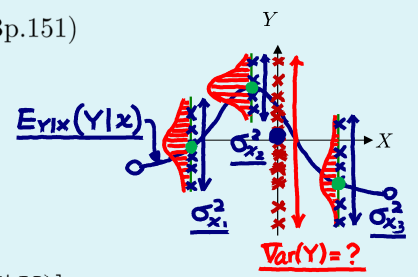
\includegraphics[width=0.8\textwidth]{image/var_dec.png}
%         \label{label_for_cross_ref_1}
%     }
%     \quad    %用 \quad 来换行
%     \subfigure[$E_{Y|X}(Y|X)$为常数]{
%     	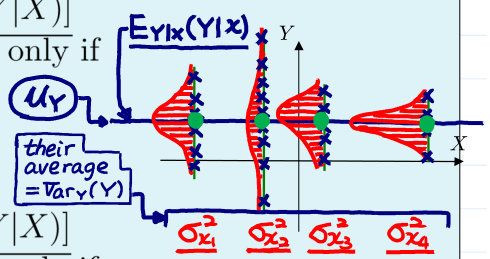
\includegraphics[width=0.4\textwidth]{image/var_dec2.png}
%         \label{label_for_cross_ref_3}
%     }
%     \subfigure[$\operatorname{Var}_{Y|X}(Y|X)=0$]{
% 	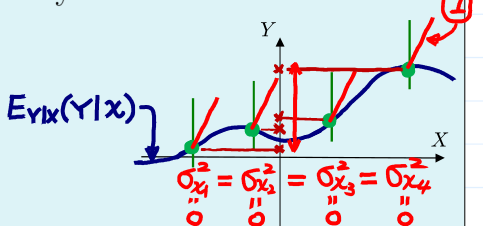
\includegraphics[width=0.4\textwidth]{image/var_dec3.png}
%         \label{label_for_cross_ref_4}
%     }
%     \caption{This is a Demo of$2\times 2$}
%     \label{fig.1}
% \end{figure}

\begin{corollary}
    \[ \operatorname{Var}_Y(Y) \ge E_X[\operatorname{Var}_{Y|X}(Y|X)] \]
    当且仅当$E_{Y|X}(Y|X)=E_Y(Y)$时取等号
\end{corollary}

\begin{corollary}
    \[ \operatorname{Var}_Y(Y) \ge \operatorname{Var}_X[E_{Y|X}(Y|X)] \]
    当且仅当$\operatorname{Var}_{Y|X}(Y|X)=0$,即$\E_{Y|X}(Y|X)=Y$时取等号
\end{corollary}

\section{矩母函数与特征函数}

\subsection{矩}

\begin{definition}
    对于随机变量$X$,定义其$k$阶\textbf{矩}(moment)为$E(X^k)$,记为$\mu_k$;定义其$k$阶\textbf{中心矩}(central moment)为$E((X-\mu_X)^k)$,记为$\upsilon_k$。
\end{definition}
由于$|X|^{k-1}\le |X|^k+1$,故$k$阶矩存在时,$k-1$阶矩也存在,从而低于$k$的各阶矩都存在.
易知矩与中心矩间存在以下关系:
\begin{align*}
    \upsilon_k & =\sum_{i=0}^k \binom{k}{i} \mu_i(-\mu_X)^{k-i}      \\
    \mu_k      & =\sum_{i=0}^k \binom{k}{i} \upsilon_i(\mu_X)^{n-i}j
\end{align*}
\begin{note}
    对于$\mu_k$做变换$E(X-\mu_X+\mu_X)^k$
\end{note}

\begin{example}
    设随机变量$X\sim N(0,\sigma^2)$,则
    \begin{align*}
        \mu_k & = E(X^k) = \frac1{\sqrt{2\pi}\sigma}\int_{-\infty}^{+\infty} x^k\ee^{-\frac{x^2}{2\sigma^2}} \dd x \\
              & = \frac{\sigma^k}{\sqrt{2\pi}} \int_{-\infty}^{+\infty}u^k\ee^{-\frac{u^2}2}\dd u.
    \end{align*}
    在$k$为奇数时,上述被积函数是奇函数,故
    \[ \mu_k = 0, k=1,3,5,\cdots \]
    在$k$为偶数时,上述被积函数是偶函数,再利用变换$z=u^2/2$,可得
    \begin{align*}
        \mu_k & = \sqrt{\frac2\pi}\sigma^k2^{(k-1)/2} \int_0^{+\infty}z^{(k-1)/2}\ee^{-z} \dd z = \sqrt{\frac2\pi}sigma^k2^{(k-1)/2} \Gamma\left( \frac{k+1}2 \right) \\
              & = \sigma^k(k-1)(k-3)\cdots1.\quad k=2,4,6,\cdots.
    \end{align*}
    故$N(0,\sigma^2)$分布的前四阶原点矩为
    \[ \mu_1 = 0,\quad \mu_2 = \sigma^2,\quad \mu_3 = 0,\quad \mu_4 = 3\sigma^4 \]
    又因为$E(X)=0$,所以有原点矩等于中心矩,即$\mu_k=\nu_k,k=1,2,\cdots$.
\end{example}

\begin{proposition}[矩存在的必要条件]
    若 $EX^k(k>0)$存在,则有
    \[ \lim_{x \to \infty}x^k[1-F(x)]=0, \quad \lim_{x \to -\infty}\abs{x}^kF(x)=0 \]
\end{proposition}
\begin{proof}
    若 $EX^k(k>0)$存在,则
    \[ E\abs{X}^k = \lim_{n \to \infty} \int_{-\infty}^{n}\abs{X}^k \d F(x) < +\infty \]
    所以
    \[ \lim_{n \to \infty}\left[ E\abs{X}^k - \int_{-\infty}^{n}\abs{X}^k \d F(x) \right]  = \lim_{n \to \infty} \int_{n}^{+\infty}\abs{X}^k \d F(x) = 0\]
    又由于
    \[ 0 \le n^k[1-F(n)] \le \int_{n}^{+\infty}\abs{X}^k \d F(x) ,\quad n>0 \]
    两边取$n \to \infty$,则可得出$\lim_{x \to \infty}x^k[1-F(x)]=0$

    同理有
    \[ \lim_{n \to -\infty} \int_{-\infty}^{n}\abs{X}^k \d F(x) = 0 \]
    及
    \[ 0 \le \abs{n}^kF(n) \le \int_{-\infty}^{n}\abs{X}^k \d F(x) ,\quad n<0 \]
    两边取$n \to -\infty$,则可得出$\lim_{x \to -\infty}\abs{x}^kF(x)=0$
\end{proof}

\subsection{矩母函数}

\begin{definition}
    对于随机变量$X$, 若下式期望存在:
    \[ M_X(t) = \E(e^{tX}) \]
    则称其为\textbf{矩母函数}(moment generating function, mgf)。
\end{definition}
\begin{remark}
    此表达式等价于对概率质量函数或密度函数作Laplace变换, 当$t$取某些特定值时, 可能不存在.(若$t=0$则永远存在)
\end{remark}

\begin{theorem}
    若当$t$属于一个包含零点的开区间时, 矩母函数一直存在, 则其唯一对应一个概率分布.
\end{theorem}

\begin{theorem}
    若当$t$属于一个包含零点的开区间时, 矩母函数一直存在, 则:
    \[ M_X^{(k)}(0) = E(X^k) \]
\end{theorem}
\begin{remark}
    借此可方便地计算各阶矩, 故称为矩母函数. 反过来, 若已知各阶矩, 通过Tayler展开$M_X(t)=\sum_{k=0}^{\infty}\frac{M_X^{(k)}(0)}{k!}t^k$可还原矩母函数, 进而得出概率分布.
\end{remark}

\begin{proposition}
    若$a,b$为常数, 则
    \[ M_{a+b X}(t) = e^{a t}M_X(b t) \]
\end{proposition}

\begin{theorem}\label{thm:mgf_sum}
    若$X,Y$独立,则
    \[ M_{X+Y}(t) = M_X(t) M_Y(t) \]

    泛化情况: 若$X_1,\cdots, X_n$相互独立,则
    \[ M_{X_1+\cdots+ X_n} = \prod_{i=1}^n M_{X_i}(t)\]
\end{theorem}

\subsection{联合特征函数}

\begin{definition}
    对于随机变量$X_1,\cdots, X_n$, 若下式期望存在:
    \[ M_{X_1\cdots X_n}(t_1,\cdots ,t_n) = \E(e^{t_1 X_1+\cdots + t_n X_n}) \]
    则称其为\textbf{联合矩母函数}(joint moment generating function, joint mgf)。
\end{definition}

\begin{remark}
    此处为\underline{多元}函数
\end{remark}

\begin{proposition}
    \[ M_{X_i}(t_i) = M_{X_1\cdots X_n}(0,\cdots ,t_i,\cdots ,0) \]
\end{proposition}

\begin{theorem}
    当且仅当:
    \[ M_{X_1\cdots X_n}(t_1,\cdots ,t_n) = \prod_{i=1}^n M_{X_i}(t_i) \]
    时,$X_1,\cdots, X_n$相互独立
\end{theorem}

\begin{remark}
    与\underline{累计函数、密度函数、质量函数}的情况类似,变量相互独立等价于联合函数可拆分为边缘函数的乘积
\end{remark}

\begin{theorem}
    \[ \frac{\partial^{r_1+\cdots +r_n} }{\partial t_1^{r_1} \cdots  \partial t_n^{r_n}} M_{X_1\cdots X_n}(t_1,\cdots ,t_n) = E(X_1^{r_1} \cdots X_n^{r_n}) \]
\end{theorem}

\subsection{特征函数}

由于有时矩母函数可能不存在,为避免此缺陷,构造出与之特性类似的特征函数。

\begin{definition}
    对于随机变量$X$, 定义其\textbf{特征函数}(characat function, chf)为:
    \[ \varphi_X(t) = \E(e^{itX}) = \E(\cos(tX)) + i\E(\sin(tX))\]

    对于随机变量$X_1,\cdots, X_n$, 定义其\textbf{联合特征函数}(joint characat function, joint chf)为:
    \[ \varphi_{X_1\cdots X_n}(t_1,\cdots ,t_n) = \E(e^{i(t_1 X_1+\cdots + t_n X_n)}) \]
\end{definition}
\begin{remark}
    此表达式等价于对概率质量函数或密度函数作Fourier变换
\end{remark}

\begin{proposition}[特征函数的性质]
    \begin{enumerate}
        \item$\lvert \varphi(t) \rvert \leq \varphi(0) = 1$,即随机变量的特征函数总是存在。
        \item 且若矩母函数存在,则其与特征函数之间满足关系:$\varphi_X(t) = M_X(it)$
              \item$\varphi(-t) = \overline{\varphi(t)}$
        \item 若$Y = aX + b$, 其中$a,b$是常数, 则
              \begin{equation}\label{eq:chf_linear}
                  \varphi_Y(t) = \ee^{ibt} \varphi_X(at).
              \end{equation}
        \item 独立随机变量和的特征函数为特征函数的积,
              即设$X$与$Y$相互独立, 则
              \begin{equation}\label{eq:chf_sum}
                  \varphi_{X+Y}(t) = \varphi_X(t) \cdot \varphi_Y(t).
              \end{equation}
        \item 若$E(x^l)$存在,
              则$X$的特征函数$\varphi(t)$可$l$次求导,
              且对$1 \leq k \leq l$, 有
              \begin{equation}\label{eq:chf_derivative}
                  \varphi^{(k)}(0) = i^k E(X^k).
              \end{equation}
    \end{enumerate}
\end{proposition}
\begin{proof}
    \begin{enumerate}
        \item
              \begin{align*}
                  |\varphi(t)| & = \left\lvert \int_{-\infty}^{+\infty} \ee^{itx} p(x) \dd x \right\rvert
                  \leq \int_{-\infty}^{+\infty} \left\lvert \ee^{itx} \right\rvert p(x) \dd x             \\
                               & = \int_{-\infty}^{+\infty} p(x) \dd x
                  = \varphi(0)
                  = 1.
              \end{align*}
        \item
              \[ \varphi(-t) = \int_{-\infty}^{+\infty} \ee^{-itx} p(x) \dd x
                  = \overline{\int_{-\infty}^{+\infty} \ee^{itx} p(x) \dd x}
                  = \overline{\varphi(t)} \]
        \item
              \[ \varphi_Y(t) = E(\ee^{it(aX + b)})
                  = \ee^{ibt} E(\ee^{iatX}) = \ee^{ibt} \varphi(at) \]
        \item 因为$X$与$Y$相互独立, 所以$\ee^{itX}$与$\ee^{itY}$也是独立的, 从而有
              \[ E \left(\ee^{it(X + Y)} \right) = E \left(\ee^{itX} \ee^{itY} \right) = \varphi_X(t) \cdot \varphi_Y(t) \]
        \item 因为$E \left(X^l \right)$存在,即
              \[ \int_{-\infty}^{+\infty} \lvert x \rvert^l p(x) \dd x < +\infty \]
              于是含参变量$t$的广义积分$\int_{-\infty}^{+\infty} \ee^{itx} p(x) \dd x$可以对$t$求导$l$次, 于是对$0 \leq k \leq l$, 有
              \[ \varphi ^{(k)}(t) = \int_{-\infty}^{+\infty} i^k x^k \ee^{itx} p(x) \dd x = i^k E \left(X^k \ee^{itX} \right) \]
              令$t = 0$即得
              \[ \varphi^{(k)}(0) = i^k E \left(X^k \right) \]
    \end{enumerate}
\end{proof}

\begin{example}[柯西分布的特征函数]\label{ex:Cauchy_dist_chf}
    对于柯西分布特征函数的求解,不妨先设$\mu=0$,则$f(x) = \frac{\sigma}{\pi} \frac1{\sigma^2+x^2}$,则其特征函数为:
    \[ \varphi(t)=\frac{a}{\pi}\int_{-\infty}^{+\infty} \frac{\ee^{itx}}{x^2+\sigma^2} \d x = \frac{2a}{\pi}\int_{0}^{+\infty} \frac{\cos t x}{x^2+\sigma^2} \d x \]
    因为当$t>0$时,
    \[ \int_{0}^{+\infty} \frac{\cos t x}{x^2+\sigma^2} \d x = \frac{\pi}{a} \ee^{-at} \]
    所以当$t>0$时,$\varphi(t)=\ee^{-\sigma t}$。当$t<0$时,$\varphi(t)=\overline{\varphi(-t)}=\ee^{\sigma t}$。即$\varphi(t)=\ee^{-\sigma |t|}$。

    对于一般情况,则$Cau(\mu,\sigma)=Cau(0,\sigma)-\mu$
    \[ \varphi(t)=\exp (i\mu t) \exp(-\sigma |t|)=\exp (i\mu t-\sigma |t|) \]
\end{example}

\begin{theorem}[逆转公式]
    设$F (x)$和$\varphi (t)$分别为随机变量$X$的分布函数和特征函数, 则对$F (x)$的任意两个连续点$x_1 < x_2$, 有
    \begin{equation}\label{eq:4.1.11}
        F (x_2) - F (x_1) = \lim_{T \to \infty} \frac{1}{2\pi} \int_{-T}^T \frac{\ee^{-itx_1}  - \ee^{-itx_2}}{it} \varphi (t) \dd t.
    \end{equation}
\end{theorem}

\begin{theorem}[唯一性定理]
    随机变量的分布函数由其特征函数唯一决定.
\end{theorem}
\begin{proof}
    对$F (x)$的每一个连续点$x$, 当$y$沿着$F (x)$的连续点趋于$-\infty$时, 由逆转公式得
    \[ F (x) = \lim_{y \to -\infty} \lim_{T \to +\infty} \frac{1}{2\pi} \int_{-T}^T \frac{\ee^{-ity} - \ee^{-itx}}{it} \varphi (t) \dd t \]
    而分布函数由其连续点上的值惟一决定(非连续点的情况可由右连续的性质推出),故结论成立.
\end{proof}

\begin{theorem}
    特征函数可通过以下逆变换得到分布:\\
    \textbf{离散情况}:
    \[ p_X(x)=\lim _{T \rightarrow \infty} \int_{-T}^{T} e^{-i t x} \varphi_X(t) \d t \]
    \textbf{连续情况}:
    \[ f_X(x)=\frac1{2 \pi} \int_{-\infty}^{\infty} e^{-i t x} \varphi_X(t) \d t \]
\end{theorem}
\begin{remark}
    此即傅里叶逆变换。
\end{remark}
\begin{proof}
    记$X$的分布函数为$F (x)$, 由逆转公式知
    \begin{align*}
        p (x) & = \lim_{\Delta x \to 0} \frac{F (x + \Delta x) - F (x)}{\Delta x}                                                                                  \\
              & = \lim_{\Delta x \to 0} \frac{1}{2\pi} \int_{-\infty}^{+\infty} \frac{\ee^{-itx} - \ee^{-it (x + \Delta x)}}{it \cdot \Delta x} \varphi (t) \dd t.
    \end{align*}
    再次利用不等式$\lvert \ee^{ia} - 1 \rvert \leq \lvert a \rvert$, 就有
    \[ \left\lvert \frac{\ee^{-itx} - \ee^{-it (x + \Delta x)}}{it \cdot \Delta x} \right\rvert \leq 1 \]
    又因为$\int_{-\infty}^{+\infty} \lvert \varphi (t) \rvert < +\infty$, 所以可以交换极限号和积分号, 即
    \begin{align*}
        p (x) & = \frac{1}{2\pi} \int_{-\infty}^{+\infty} \lim_{\Delta x \to 0} \frac{\ee^{-itx} - \ee^{-it (x + \Delta x)}}{it \cdot \Delta x} \varphi (t) \dd t \\
              & = \frac{1}{2\pi} \int_{-\infty}^{+\infty} \ee^{-itx} \varphi (t) \dd t.
    \end{align*}
\end{proof}

\section{估计与预测}

\subsection{delta法}

\subsection{预测}

\section{熵与信息}

\subsection{费尔希信息量}

\section{其他特征}

\subsection{变异系数}

\begin{definition}[变异系数]
    设随机变量$X$的二阶矩存在,则称比值
    \[ C_v(X) = \frac{\sqrt{\Var(X)}}{E(X)} = \frac{\sigma(X)}{E(X)} \]
    为$X$的\textbf{变异系数}
\end{definition}

因为变异系数是以其数学期望为单位去度量随机变量取值波动程度的特征数,标准差的量纲与数学期望的量纲是一致的,所以变异系数是一个无量纲的量。

\subsection{分位数}

\begin{definition}[分位数]
    设连续随机变量$X$的分布函数为$F(x)$,密度函数为$p(x)$. 对任意$p\in(0,1)$,称满足条件
    \[ F(x_p) = \int_{-\infty}^{x_p}p(x)\dd x = p \]
    的$x_p$为此分布的\textbf{$p$分位数},又称\textbf{下侧$p$分位数}.

    称满足条件
    \[ 1 - F(x_p') = \int_{x_p'}^{+\infty} p(x)\ dd x = p \]
    的$x_p'$为此分布的\textbf{上侧$p$分位数}
\end{definition}

分位数$x_p$是把密度函数下的而积分为两块,左侧面积恰好为$p$(见图 \ref{fig2.7.1}(a))。上侧分位数$x_p'$也是把密度函数下的面积分为两块,但右侧面积恰好为$p$(见图 \ref{fig2.7.1}(b)).

\begin{figure}[!ht]
    \centering
    \subfloat[(下侧)分位数]{
        \begin{tikzpicture}[thick]
            \draw[-Stealth](0,0) --(5,0) node [below] {$x$};
            \fill[pattern = north west lines](0,0) .. controls(0.5,0.6) ..(1,2.2) --(1,0) -- cycle;
            \draw(0,0).. controls(0.5,0.6) ..(1,2.2) [bend left = 38] to(1.5,2.6) [bend left = 30] to(2.2,2) [bend right = 30] to(4.9,0.1);
            \draw [densely dashed](1,0) node[below]{$x_p$} --(1,2.2);

            \node[inner sep=0pt, circle ,fill = white] at(0.7,0.4){$p$};
            \draw[-Stealth](4,1.5) node[above] {$p(x)$} -- ++(-135:1.1);
        \end{tikzpicture}
    }\qquad
    \subfloat[上侧分位数]{
        \begin{tikzpicture}[thick]
            \draw[-Stealth](0,0) --(5,0) node [below] {$x$};
            \fill[pattern = north east lines](2.2,2) [bend right = 30] to(4.9,0.1) --(4.9,0) --(2.2,0) node[below]{$x_p'$} -- cycle;
            \draw(0,0).. controls(0.5,0.6) ..(1,2.2) [bend left = 38] to(1.5,2.6) [bend left = 30] to(2.2,2) [bend right = 30] to(4.9,0.1);
            \draw [densely dashed](2.2,0) --(2.2,2);
            \node[inner sep=0pt, circle ,fill = white] at(3,0.4){$p$};
            \draw[-Stealth](4,1.5) node[above] {$p(x)$} -- ++(-135:1.1);
        \end{tikzpicture}
    }
    \caption{分位数与上侧分位数的区别\label{fig2.7.1}}
\end{figure}

分位数与上侧分位数是可以相互转换的,其转换公式如下.
\begin{equation}
    x_p' = x_{1-p};\quad x_p = x_{1-p}'.
\end{equation}

\begin{definition}[中位数]
    设连续随机变量$X$的分布函数为$F(x)$,密度函数为$p(x)$.称$p=0.5$时的$p$分位数$x_{0.5}$为此分布的\textbf{中位数},即$x_{0.5}$满足
    \[ F_(x_{0.5}) = \int_{-\infty}^{0.5} p(x) \dd x = 0.5 \]
\end{definition}

\begin{figure}[!ht]
    \centering
    \begin{tikzpicture}
        \draw [-Stealth](-0.5,0) --(0,0)node[below left] {$O$} --(4.5,0) node[below]{$x$};
        \draw [-Stealth](0,-0.5) --(0,1.2) node [left]{0.5} --(0,3) node[left]{$F(x)$};
        \draw [densely dashed](0,2.4) -- ++(3.8,0)
        (1.5,0)node[below]{$x_{0.5}$} --(1.5,1.2)
        --(0,1.2);

        \draw [thick](-0.5,0.1) [bend right=30] to(1.5,1.2) [bend left=30] to(3.6,2.3);
    \end{tikzpicture} \quad
    \begin{tikzpicture}
        \draw [-Stealth](-0.5,0) --(0,0)node[below left] {$O$} --(4.5,0) node[below]{$x$};
        \draw [-Stealth](0,-0.5) -- (0,3) node[left]{$p(x)$};
        \draw [thick](-0.5,0) [bend right = 20] to(0,0.7) [bend left = 10] to(0.6,2.1)[bend left=30] to(1.1,2.3) [bend left = 30] to(1.8,1.8)[bend right = 35] to(4,0.2);
        \fill [pattern = north east lines](-0.5,0) [bend right = 20] to(0,0.7) [bend left = 10] to(0.6,2.1)[bend left=30] to(1.1,2.3) --(1.1,0) node [below]{$x_{0.5}$} -- cycle;
        \fill [pattern = north west lines] (1.1,2.3) [bend left = 30] to(1.8,1.8)[bend right = 35] to(4,0.2) --(4.3,0) --(1.1,0) -- cycle;
        \draw(0.6,0.6) node[fill=white,circle,inner sep=0pt] {0.5}(1.8,0.6)node[fill=white,circle,inner sep=0pt]{0.5};
        \draw [-Stealth](3,1.7)node[above]{$p(x)$} -- ++(-135:1);
    \end{tikzpicture}
    \caption{连续随机变量的中位数\label{fig2.7.2}}
\end{figure}

\subsection{偏度系数与峰度系数}

\begin{definition}[偏度系数]
    设随机变量$X$的三阶矩存在,则称比值
    \[ \beta_1 = \frac{E[X-E(X)]^3}{[E(X-E(X))^2]^{3/2}} = \frac{\nu_3}{(\nu_2)^{3/2}} \]
    为$X$的分布的\textbf{偏度系数},简称\textbf{偏度}.
\end{definition}

偏度系数可以描述分布的形状特征,其取值的正负反映的是

\begin{itemize}
    \item 当$\beta_1>0$时,分布为正偏或右偏
    \item 当$\beta_1=0$时,分布关于其均值$E(X)$对称
    \item 当$\beta_1<0$时,分布为负偏或左偏
\end{itemize}

\begin{figure}[!ht]
    \centering
    \subfloat[]{
        \begin{tikzpicture}
            \draw [-Stealth](0,0) node[below left]{$O$} --(2,0) node [below]{$\beta_1>0$} --(4,0) node[below]{$x$};
            \draw [-Stealth](0,0) --(0,4) node [right]{$p(x)$};
            \draw [thick](0,0) [bend left = 10] to(0.8,2.6) [bend left = 42] to(1.4,2.8)
            [bend left = 23] to(1.51,2.65) [bend right = 15] to(2.8,0.5) [bend right =13] to(3.5,0.1);
        \end{tikzpicture}
    }\;
    \subfloat[]{
        \begin{tikzpicture}
            \draw [-Stealth](-0.4,0) node[below left]{$O$} --(4,0) node[below]{$x$};
            \draw [-Stealth](0,0) --(0,4) node [right]{$p(x)$};
            \draw[thick](-0.3,0.1) [bend right = 25] to(1.2,2.4) [bend left = 15] to(1.5,3.1)
            [bend left=55] to(1.7,3.1) [bend left =10] to(1.9,2.2) [bend right=30] to(3.5,0.1);

            \draw [thick,densely dashed](1.6,3.15) --(1.6,0) node[below] {$\beta_1=0$};
        \end{tikzpicture}
    }\;
    \subfloat[]{
        \begin{tikzpicture}
            \draw [-Stealth](0,0) node[below left]{$O$} --(2,0) node [below]{$\beta_1<0$} --(4,0) node[below]{$x$};
            \draw [-Stealth](0,0) --(0,4) node [right]{$p(x)$};
            \draw [thick](0.2,0.1) [bend right=25] to(2.4,2.6) [bend left=19] to(2.6,2.9) [bend left=30] to(2.8,2.9) [bend left=20] to(2.9,2.7)
            [bend right=10] to(3.6,0.2) [bend right=25] to(3.8,0.01) ;
        \end{tikzpicture}
    }
    \caption{三种不同偏度的分布}
\end{figure}

譬如,正态分布$N(\mu,\sigma^2)$是关于其均值$E(X)=\mu$是对称的,所以正态分布的偏度$\beta_1=0$.

\begin{definition}[峰度系数]
    设随机变量$X$的四阶矩存在,则称比值
    \[ \beta_2 = \frac{E[X-E(X)]^4}{[E(X-E(X))^2]^2} - 3 = \frac{\nu_4}{(\nu_2)^2} -3 \]
    为X的分布的\textbf{峰度系数},简称\textbf{峰度}.
\end{definition}

峰度系数也是用于描述分布的形状特征,但峰度系数与偏度系数的差别是:偏度系数刻画的是分布的对称性,而峰度系数刻画的是分布的蜂峭性.

峰度系数把正态分布的峰峭性作为标准,因为正态分布$N(\mu,\sigma^2)$的四阶中心矩为$\nu_4=3\sigma^4$,所以其峰度系数为
\[ \beta_2 = \frac{\nu_4}{(\nu_2)^2} - 3 = \frac{3\sigma^4}{\sigma^4} - 3 = 0 \]
这说明:任一正态分布的峰度$\beta_2=0$.

可见,这里谈论的“峰度”不是指密度函数的峰值高低,那么“蜂度”的含义到底是什么呢?或者换句话说,我们应该如何刻画密度函数的峰峭性呢?我们知道从图形上看密度函数曲线下的面积等于1,若随机变量取值较集中,则其密度函数的峰值必高无疑,所以密度函数峰值的高低含有随机变量取值的集中程度.为了消除这个因素,我们不妨考察“标准化”后的分布的峰峭性,即用
\[ X^\ast = \frac{X - E(X)} {\sqrt{\Var(X)}} \]
的四阶原点矩$E[(X^\ast)^4]$考察密度函数的峰值,再考虑到任一标准正态分布的四阶原点矩等于3,所以就有了以上峰度系数的定义.

综上所述,一个分布的峰度系数$\beta_2$反映了以下情况:
\begin{itemize}
    \item 当$\beta_2<0$时,则标准化后的分布形状比标准正态分布更平坦,称为\textbf{低峰度}.
    \item 当$\beta_2=0$时,则标准化后的分布形状与标准正态分布相当.
    \item 当$\beta_2>0$时,则标准化后的分布形状比标准正态分布更尖峭,称为\textbf{高峰度}.
\end{itemize}


\begin{problemset}[错题记录]
    \item (茆2.2.7)对一批产品进行检查,如查到第$a$件全为合格品,就认为这批产品合格;若在前$a$件中发现不合格品即停止检查,且认为这批产品不合格。设产品的数量很大,可认为每次查到不合格品的概率都是$p$。问每批产品平均要查多少件?
    \item (茆2.2.17)设随机变量$X$的概率密度函数为
    \[ p(x)=\begin{cases}
            \frac{1}{2} \cos \frac{x}{2}, & 0 \leq x \leq \pi; \\
            0,                            & \text{其他}.
        \end{cases} \]
    对$X$独立重复观察4次,$Y$表示观察值大于$\pi/3$的次数,求$Y^2$的数学期望。
    \item (茆2.2.20)设连续随机变量$X$的分布函数为$F(x)$,且数学期望存在,证明
    \[ E(X) = \int_{0}^{+\infty}[1-F(x)] \dd  x-\int_{-\infty}^{0} F(x) \dd  x \]
    \item (茆2.2.21)设$X$是非负连续随机变量,若$E(X^n)$存在,证明:\begin{enumerate}
        \item$E(X)=\int_0^{\infty}P(X>x) \mathrm{d}x$
        \item$E(X^n)=\int_0^{\infty}n x^{n-1}P(X>x) \mathrm{d}x$
    \end{enumerate}
    \item (茆2.2.22)甲、乙两人进行象棋比赛,每局甲胜的概率为$p$,乙胜的概率为$q=1-p$。比赛进行到有一人连胜两局为止,求平均比赛局数。
    \item (茆2.2.23)设随机变量$X$的分布函数为
    \[ F(x)=\begin{cases}
            0,                                  & x<-1         \\
            \frac{1}{2}+\frac{1}{\pi}\arcsin x, & -1\le x\le 1 \\
            1,                                  & x\ge 1
        \end{cases} \]
    试求$E(X)$。
    \item (茆3.4.2)求掷$n$颗骰子出现点数之和的数学期望与方差.
    \item (茆3.4.4)设在区间$(0,1)$上随机地取$n$个点, 求相距最远的两点间的距离的数学期望.
    \item (茆3.4.10)设随机变量$X$与$Y$独立同分布,且$E(X)=\mu, \Var(X)=\sigma^2$,试求$E(X-Y)$。
    \item (茆3.4.13)系统由$n$个部件组成. 记$X_i$为第$i$个部件能持续工作的时间, 如果$X_1,\ldots,X_n$独立同分布, 且$X_i\sim Exp(\lambda)$,如果至少有一个部件在工作, 系统就工作求系统持续工作的平均时间。
    \item (茆3.4.17)一商店经销某种商品, 每周进货量$X$与顾客对该种商品的需求量$Y$是相互独立的随机变量, 且都跟从区间$(10,20)$上的均匀分布. 商店每售出一单位商品可得利润$1000$元; 若需求量超过了进货量, 则可从其他商店调剂供应, 这时每单位商品获利润为$500$元. 试求此商店经销该种商品每局的平均利润.
    \item (茆3.4.21)掷一颗骰子两次,求其点数之和与点数之差的协方差。
    \item (茆3.4.26)设随机变量$X$和$Y$的数学期望分别为$-2$和$2$,方差分别为$1$和$4$,而它们的相关系数为$-0.5$。试根据车比晓夫不等式,估计$P(|X+Y|\ge 6)$的上限。
    \item (茆3.4.29)已知随机变量$X$与$Y$的相关系数为$\rho$,求$X_1=aX+b$与$Y_1=cY+d$的相关系数,其中$a,b,c,d$均为常数。
    \item (茆3.4.32)设二维随机变量$(X,Y) \sim N(0,0,1,1,\rho)$
    \begin{enumerate}
        \item 求$E[\max(X,Y)]$
        \item 求$X-Y$与$XY$的协方差及相关系数
    \end{enumerate}
    \item (茆3.4.34)设二维随机变量$(X,Y)$的联合密度函数为
    \[ f(x,y)=\begin{cases}
            \frac{6}{7}\left(x^2+\frac{xy}{2} \right), & 0<x<1,0<y<2; \\
            0,                                         & \text{其他}.
        \end{cases} \]
    求$X$与$Y$的协方差及相关系数.
    \item (茆3.4.36)设二维随机变量$(X,Y)$的联合密度函数如下,试求$(X,Y)$的协方差矩阵。
    \[ f(x,y)=\begin{cases}
            \frac{x+y}{8}, & 0<x<2,0<y<2  \\
            0,             & \text{其他}.
        \end{cases} \]
    \item (茆3.4.38)设随机向量$(X_1,X_2,X_3)$满足条件
    \begin{align*}
         & aX_1+bX_2+cX_3=0,                       \\
         & E(X_1)=E(X_2)=E(X_3)=d,                 \\
         & \Var(X_1)=\Var(X_2)=\Var(X_3)=\sigma^2.
    \end{align*}
    其中$a, b, c, d, \sigma^{2}$均为常数,求相关系数$\rho_{12},\rho_{23},\rho_{31}$.
    \item (茆3.4.39)设随机向量$X$与$Y$都只能取两个值,试证:$X$与$Y$的独立性与不相关性是等价的。
    \item (茆3.4.42)设随机向量$(X_1,X_2,X_3)$的相关系数为$\rho_{12},\rho_{23},\rho_{31}$,证明
    \[ \rho_{12}^{2}+\rho_{23}^{2}+p_{31}^{2} \le 1+2 \rho_{12} \rho_{23} \rho_{31} \]
    \item (茆3.4.46)设二维随机向量$(X,Y)$服从二维正态分布,且
    \[ E(X)=E(Y)=0, \quad E(X Y)<0. \]
    证明: 对任意正常数$a,b$有
    \[ P(X \ge a, Y \ge b) \le P(X \ge a) P(Y \ge b) \]
    \item (茆3.4.47-52)
    \item (茆3.5.4)设随机变量$X$与$Y$独立同分布,试在以下情况下求$P(X=k|X+Y=m)$
    \begin{itemize}
        \item X与Y都服从参数为p的几何分布
        \item X与Y都服从参数为(n,p)的二项分布.
    \end{itemize}
    \item (茆3.5.9)设随机变量$X$服从$(1,2)$上的均匀分布,在$X=x$的条件下,随机变量$Y$的条件分布是参数为$x$的指数分布,证明:$XY$服从参数为$1$的指数分布。
    \item (茆4.2.5)设$X \sim N ( \mu, \sigma^2 )$,试用特征函数的方法求$X$的3阶及4阶中心矩。
    \item (茆4.2.12)设连续随机变量$X$的密度函数为$p(x)$,试证:$p (x)$关于原点对称的充要条件是它的特征函数是实的偶函数。
    \item (李5.13)
\end{problemset}
